\section{Simulation Analysis}
\label{sec:simulation}

\subsection{Operating Point Analysis for t$<$0}

\par Table~\ref{tab:op_tb0} shows the simulated operating point results for the circuit
under analysis, when t$<$0.

\begin{table}[H]
  \centering
  \begin{tabular}{|l|r|}
    \hline    
    {\bf Name} & {\bf Value [A or V]} \\ \hline
    c[i] & 0.000000e+00\\ \hline
gib[i] & -2.26373e-04\\ \hline
r1[i] & 2.161226e-04\\ \hline
r2[i] & -2.26373e-04\\ \hline
r3[i] & -1.02499e-05\\ \hline
r4[i] & 1.194589e-03\\ \hline
r5[i] & -2.26373e-04\\ \hline
r6[i] & 9.784660e-04\\ \hline
r7[i] & 9.784660e-04\\ \hline
v(1) & 5.125627e+00\\ \hline
v(2) & 4.903891e+00\\ \hline
v(3) & 4.446215e+00\\ \hline
v(4) & -1.97572e+00\\ \hline
v(5) & 4.934963e+00\\ \hline
v(6) & 5.635816e+00\\ \hline
v(7) & -1.97572e+00\\ \hline
v(8) & -2.98275e+00\\ \hline

  \end{tabular}
  \caption{Operating point. A variable followed by [i] or [current] is of type {\em current}
    and expressed in Ampere; other variables are of type {\it voltage} and expressed in
    Volt.}
  \label{tab:op_tb0}
\end{table}

\par  As we can see, the simulation results are similar to the ones we obtained in the section \ref{sec:analysis}, concerning both the numerical values and the directions. As expected, the current through the capacitor is $i_c=0$.

\newpage
\subsection{Analysis for t=0}
\label{subsec:t0}  


\par Table~\ref{tab:op_vs0} shows the simulated operating point results for the circuit
under analysis,  when t=0.
\begin{table}[H]
  \centering
  \begin{tabular}{|l|r|}
    \hline    
    {\bf Name} & {\bf Value [A or V]} \\ \hline
    gib[i] & 6.327120e-18\\ \hline
r1[i] & -6.04063e-18\\ \hline
r2[i] & 6.327120e-18\\ \hline
r3[i] & 2.864858e-19\\ \hline
r4[i] & 1.289989e-18\\ \hline
r5[i] & -2.78376e-03\\ \hline
r6[i] & 1.301043e-18\\ \hline
r7[i] & 2.625374e-18\\ \hline
v(1) & 0.000000e+00\\ \hline
v(2) & 6.197538e-15\\ \hline
v(3) & 1.898958e-14\\ \hline
v(4) & -2.62707e-15\\ \hline
v(5) & 5.329071e-15\\ \hline
v(6) & 8.618561e+00\\ \hline
v(7) & -2.62707e-15\\ \hline
v(8) & -5.32907e-15\\ \hline

  \end{tabular}
  \caption{Operating point. A variable followed by [i] or [current] is of type {\em current}
    and expressed in Ampere; other variables are of type {\it voltage} and expressed in
    Volt.}
  \label{tab:op_vs0}
\end{table}


When t=0, the voltage $v_s$ drops to the value $v_s=0$, resulting in a discontinuity. However, because $i_c=\frac{dv_c}{dt}$, the voltage in the capacitor must be continuous for $t=0-, t=0, t=0+$, otherwise, the current $i_c$ would be infinite. Taking this into account, we replaced the capacitor with a voltage source $V_x=V_6(0-)-V_8(0-)$ that ensures this continuity. Note that, as whe can see in the table, the values of $V_6$ and $V_8$ in the nodes suffered a discontinuity in order to maintain $v_c$. 

The values obtained in simulation for t=0 are also similar to the ones we get from theoretical analysis in subsection \ref{subsec:t=0}.

\newpage
\subsection{Analysis for t$>$0 - Natural Solution}

\par Figure~\ref{fig:trans_nat} shows the plot of the natural solution for $v_6$, when t$>$0.

\begin{figure}[H] \centering
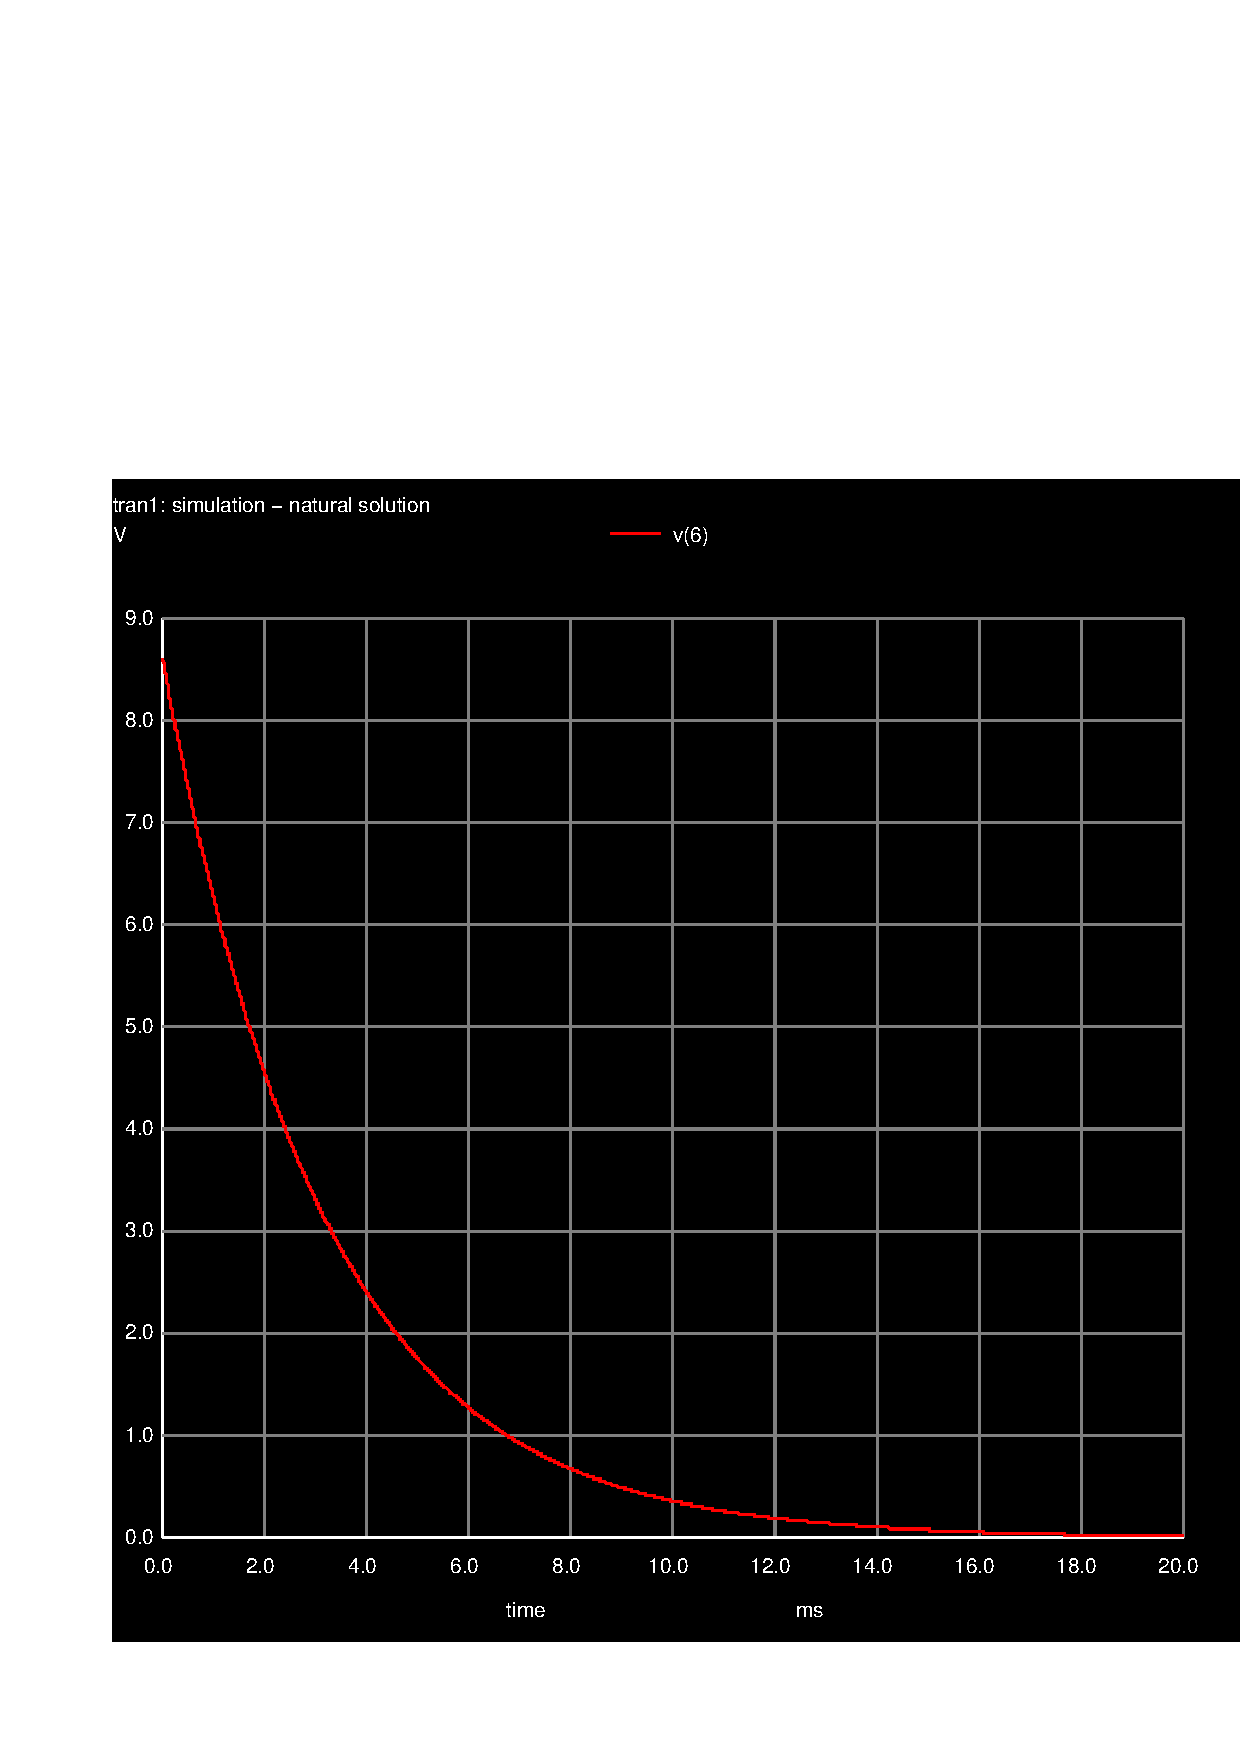
\includegraphics[clip, trim=1.3cm 1.3cm 0cm 7cm, width=0.6\linewidth]{trans_nat.pdf}
\caption{Natural solution}
\label{fig:trans_nat}
\end{figure}

To simulate the natural solution, we imposed the boundary conditions for continuity obtained in last section, $V_6$ and $V_8$, with the voltage source $v_s=0$. As we can see, the plot is similar to the one obtained in subsection \ref{subsec:nat}, showing a negative exponential.

\newpage
\subsection{Analysis for t$>$0 - Total Solution}

\par Figure~\ref{fig:trans_nat} shows the plot of the total (natural+forced) solution for $v_6$ and $v_s$, when t$>$0. Here we defined $v_s(t)=sin(2*\pi*f*t)$ as the voltage source. The plot is similar to the one obtained in subsection \ref{subsec:total_solution}.

\begin{figure}[H] \centering
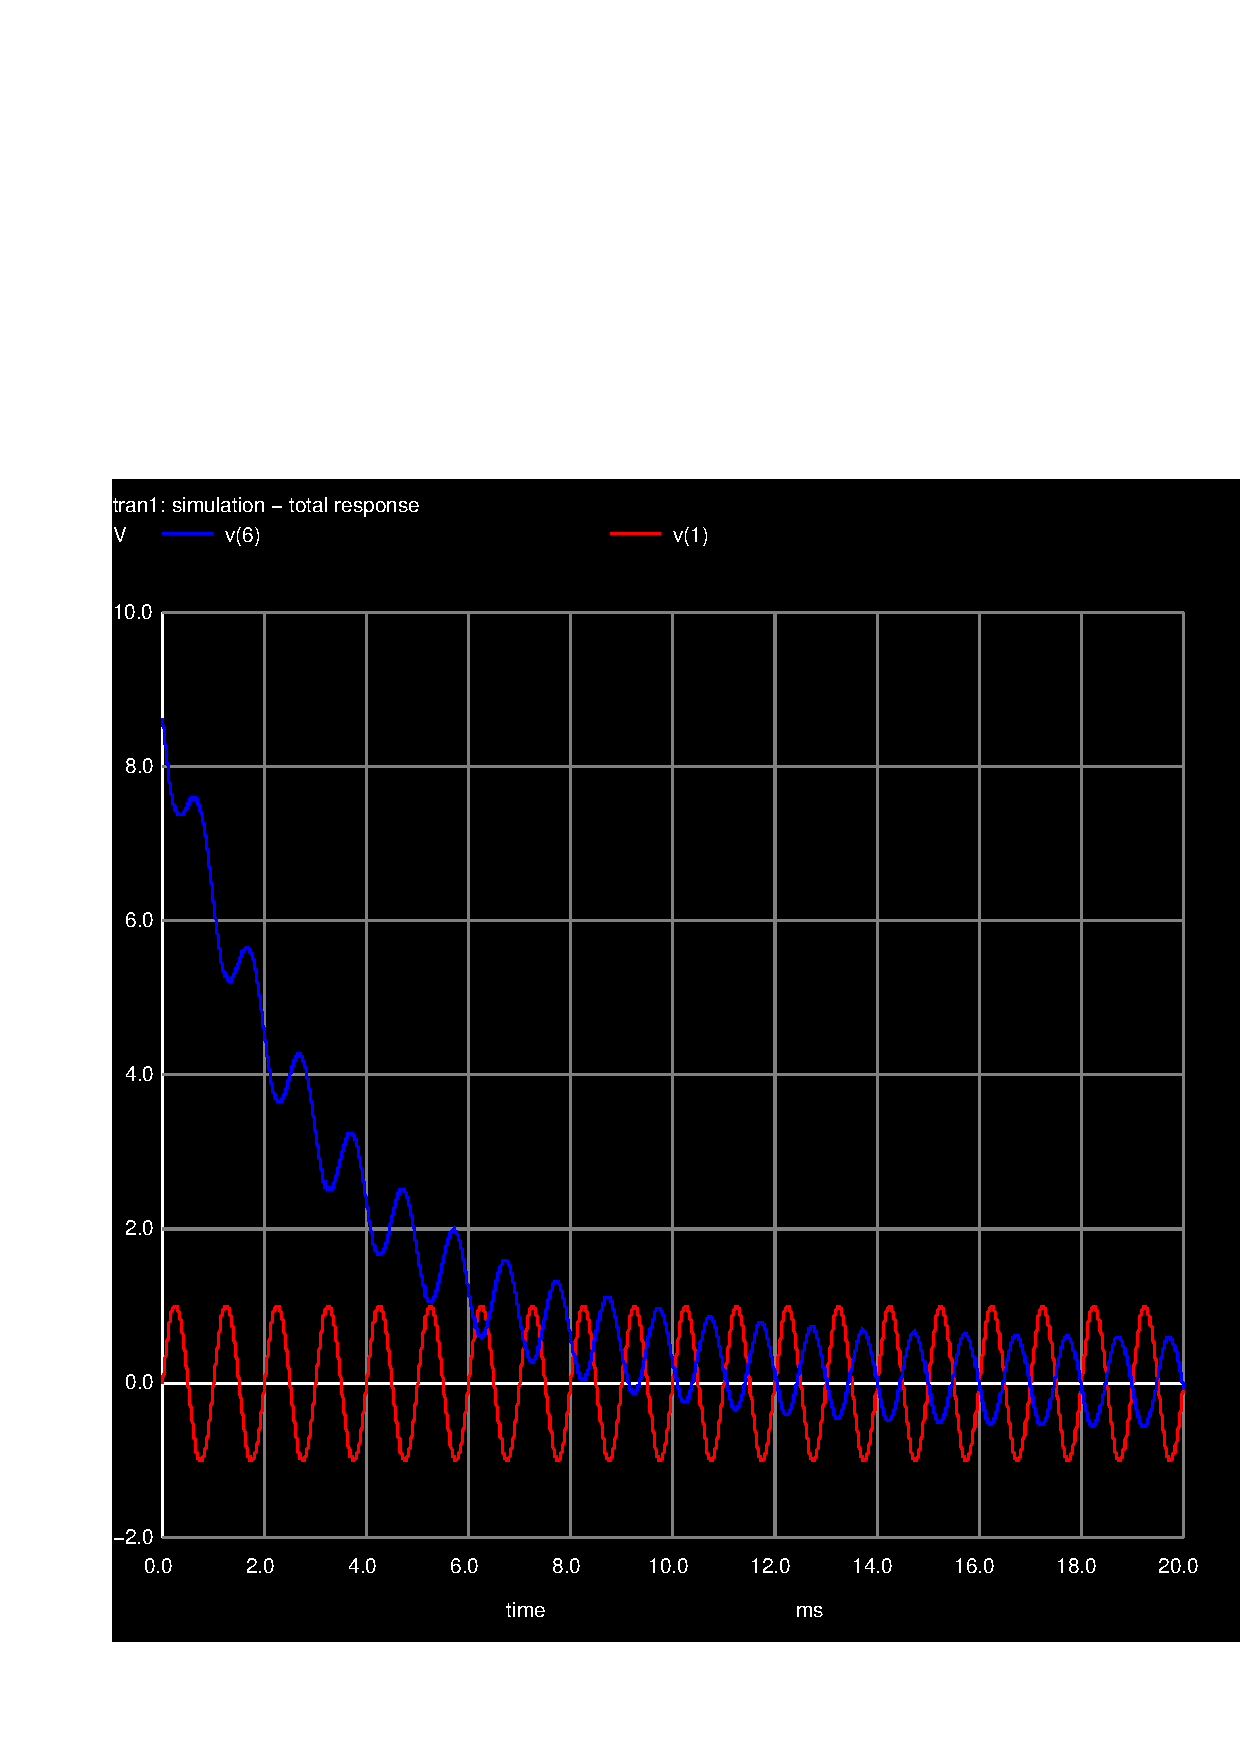
\includegraphics[clip, trim=1.3cm 1.3cm 0cm 7cm, width=0.6\linewidth]{trans_tot.pdf}
\caption{Total solution of the voltage source and the capacitor}
\label{fig:trans_tot}
\end{figure}

\newpage
\subsection{Frequency Response}

\par In this section we simulated the frequency response of $v_s$, $v_6$ and $v_c=v_6-v_8$ from frequency $0.1 Hz$ to $1 MHz$. The plot \ref{fig:magnitude} shows the magnitude response while plot \ref{fig:phase} shows the phase response. The plots are similar to the ones obtained in subsection \ref{subsec:frequency_response}\par

\begin{figure}[H] \centering
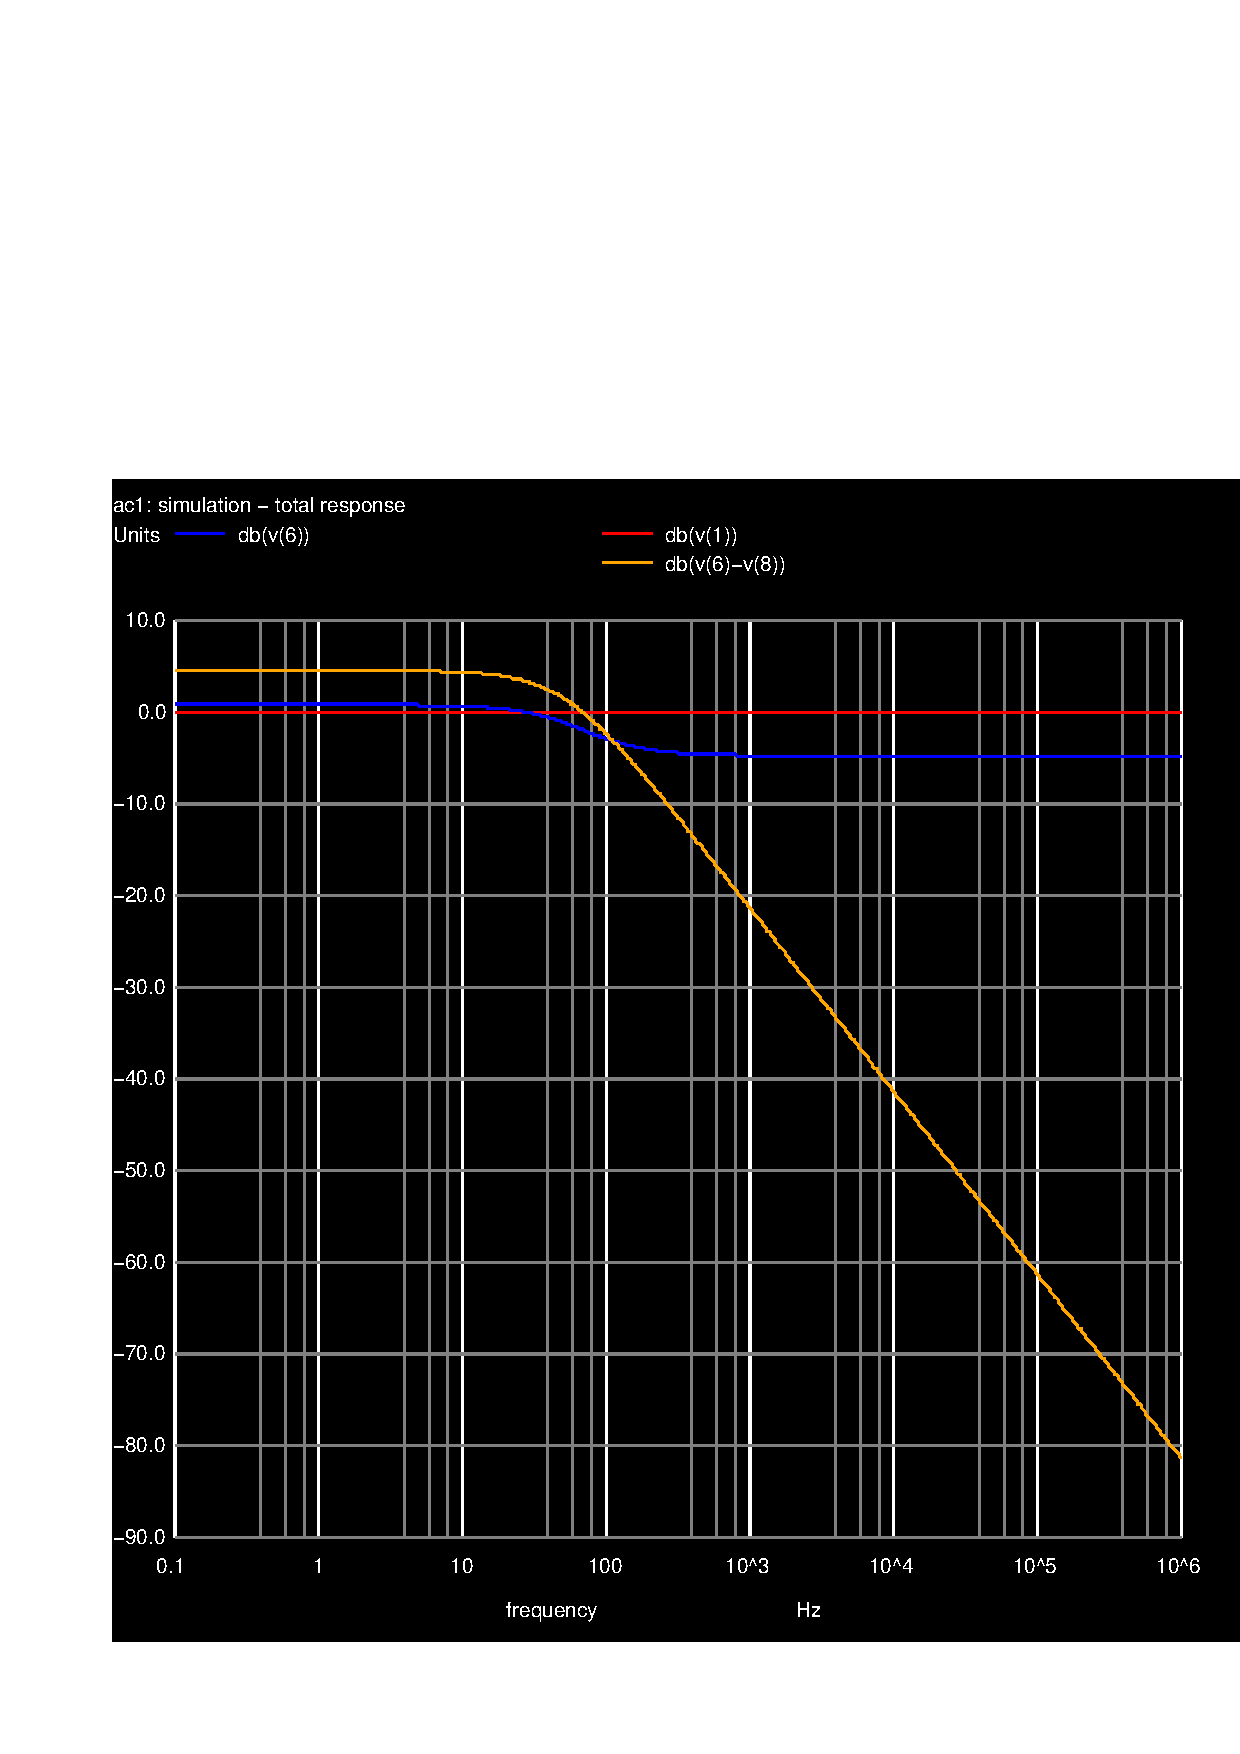
\includegraphics[clip, trim=1.3cm 1.3cm 0cm 7cm, width=0.55\linewidth]{freq_db.pdf}
\caption{Magnitude in frequency response}
\label{fig:magnitude}
\end{figure}

\begin{figure}[H] \centering
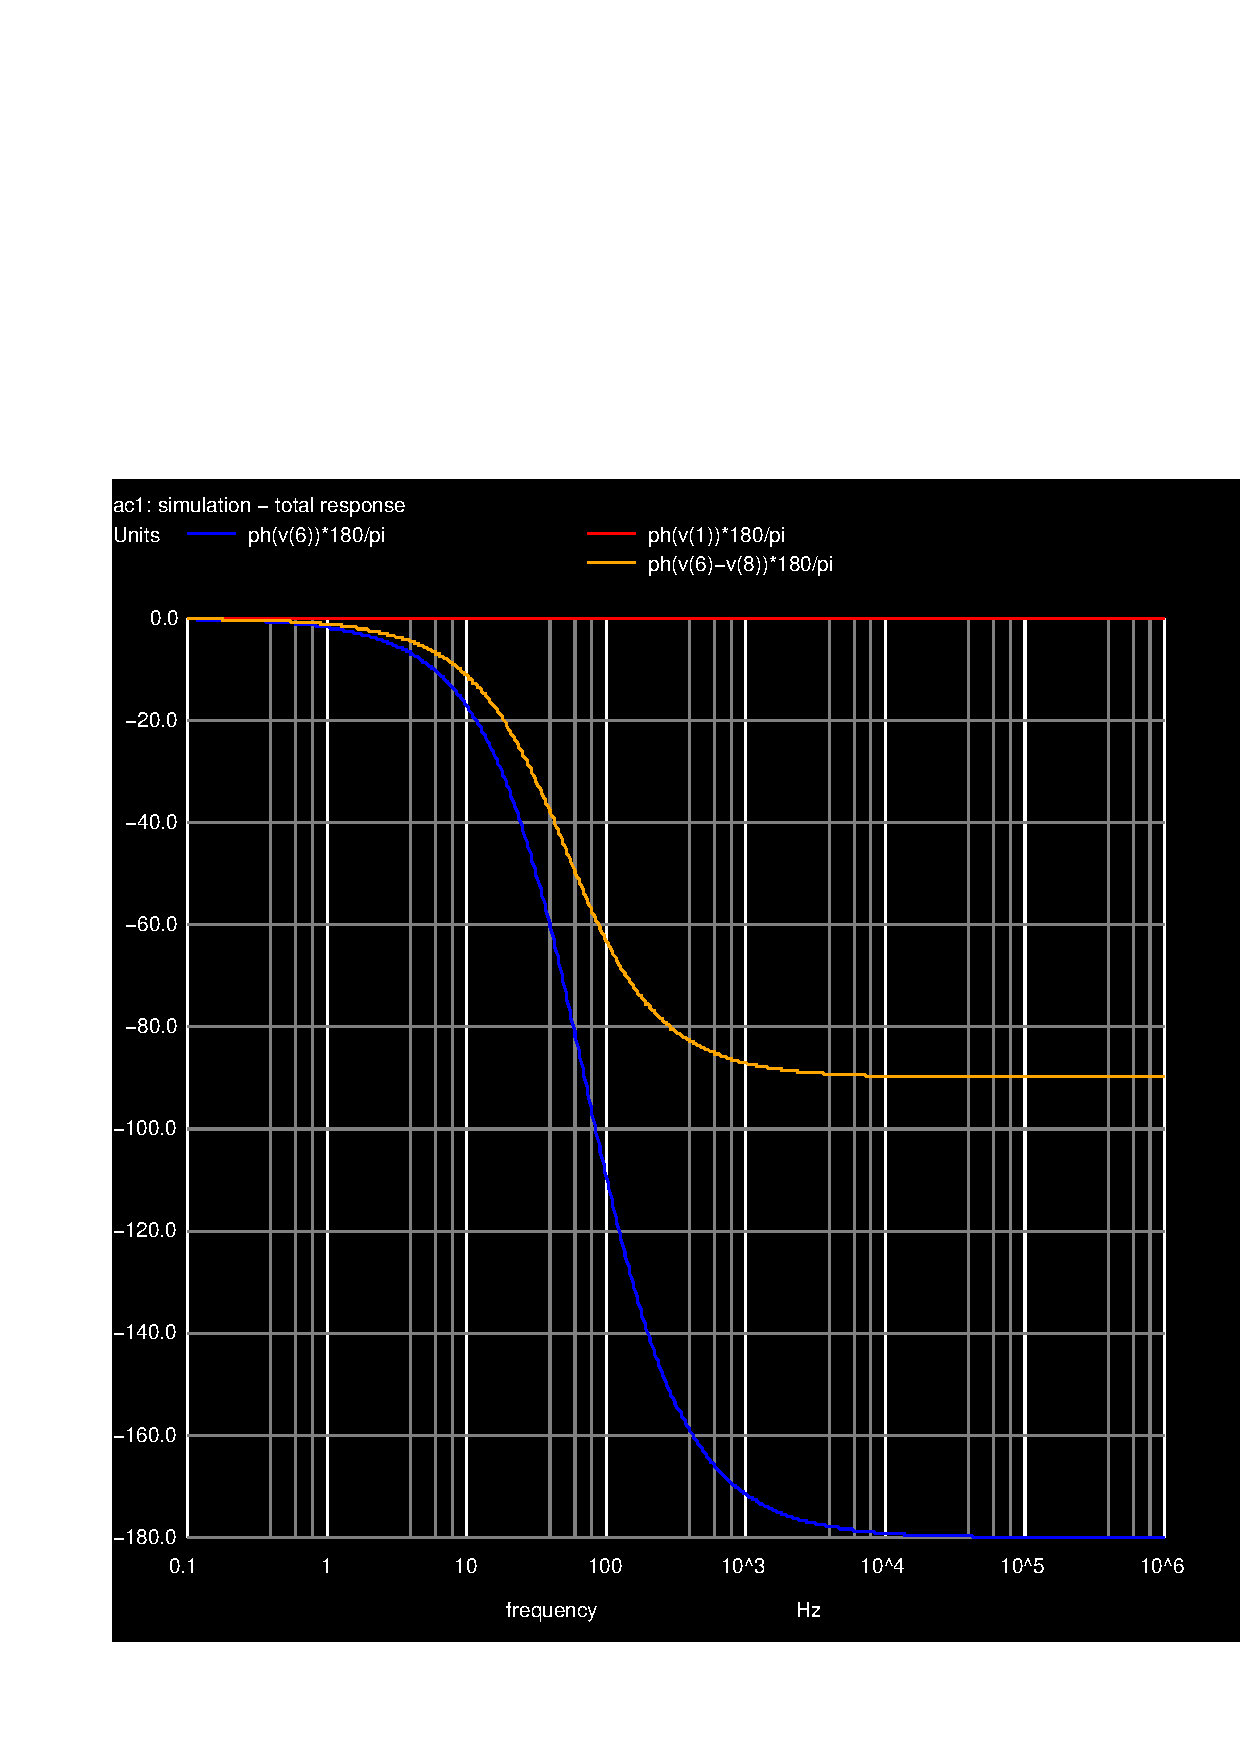
\includegraphics[clip, trim=1.3cm 1.3cm 0cm 7cm, width=0.55\linewidth]{freq_ph.pdf}
\caption{Phase in frequency response}
\label{fig:phase}
\end{figure}




